\documentclass[aspectratio=169, UTF8]{beamer}
\usepackage{math214}
\usepackage{babel}
\usepackage{tikz}
\usepackage{tikz-3dplot}
\usepackage{graphicx}
\usepackage{amsmath}

\usetheme{default}
%\usepackage{enumitem}
% Then, after \begin{document}, you can begin your frames/slides

\title{\LARGE 255RC4}
\author{Chengyang Shi, Ruizhi Deng, Haoran Shen, Jingfan Tang}
\date{Summer 2025}

\definecolor{darkblue}{HTML}{6666dd} 
\colortheme{green!30!black}
%\colortheme{orange!85!black}
%\colortheme{darkblue}
%\colortheme{blue!100!black}
%\colortheme{orange!85!white!90!black}
\begin{document}

\maketitle

%\begin{frame}
 %  \frametitle{}
  %  \tableofcontents     % 生成目录
%\end{frame}


\begin{frame}{Contents}
    \begin{enumerate}
        \item \hyperlink{2}{Lagrange Multiplier}
        \item \hyperlink{2}{Double Integrals}
        \item \hyperlink{3}{Triple Integrals}
        % \item \hyperlink{3}{Vector Field}
    \end{enumerate}
       
\end{frame}

    

\section{Lagrange Multiplier}
\begin{frame}{One Constraint}
    \frametitle{One Constraint}
    \begin{block}{Problem}
        Let $f(x, y, z)$ be a differentiable function. Suppose that we wish to find the maximum or minimum value of $f(x, y, z)$ subject to the constraint $g(x, y, z) = k$ where $k = \text{const} \in \mathbb{R}$. In other words, we wish to find the \textbf{maximum} or \textbf{minimum value} of $f(x, y, z)$ that lies on the curve $C$ described by $g(x, y, z) = k$.
    \end{block}
    \begin{block}{Solution}
        \begin{enumerate}
            \item Find all values of $x, y, z$ and $\lambda$ such that
        \[
        \boxed{\nabla f(x, y, z) = \lambda \nabla g(x, y, z), \quad g(x, y, z) = k.}
        \]
            \item Evaluate $f$ at all the points $(x, y, z)$ that result from step (1). The largest of these values is the maximum value of $f$; the smallest is the minimum value of $f$.
        \end{enumerate}
        
    \end{block}
\end{frame}
\begin{frame}{One Constraint}
    \frametitle{One Constraint}
    \textbf{Exercise} \\
    If \(\frac{x^2}{a^2} + \frac{y^2}{b^2} + \frac{z^2}{c^2} = 1\), calculate the maximum of \(f(x, y, z) = 8xyz\)
\end{frame}
\begin{frame}{Two Constraints}
    \frametitle{Two Constraints}
    \begin{block}{Problem}
        The goal is to find the \textbf{maximum and minimum values} of a three-variable function, $f(x, y, z)$, when the variables are subject to \textbf{two separate constraints}:

\begin{enumerate}
    \item $g(x, y, z) = k$
    \item $h(x, y, z) = c$
\end{enumerate}

Geometrically, this means you're looking for the extreme values of $f$ not just on a surface, but on the \textbf{curve C} where the two constraint surfaces intersect.
    \end{block}
    \begin{block}{Solution}
        \begin{enumerate}
            \item $\nabla f(x_0, y_0, z_0) = \lambda \nabla g(x_0, y_0, z_0) + \mu \nabla h(x_0, y_0, z_0)$
            \item $g(x, y, z) = k$
            \item $h(x, y, z) = c$
        \end{enumerate}
    \end{block}
\end{frame}
\begin{frame}{Two Constraints}
    \frametitle{Two Constraints}
    \begin{block}{Exercises}
        Find the maximum and minimum values of $f$ subject to the given constraints
        $f(x, y, z) = x^2 + y^2 + z^2; \quad x - y = 1, \quad y^2 - z^2 = 1$
    \end{block}
\end{frame}
\begin{frame}{Two Constraints}
    \frametitle{Two Constraints}
    \begin{block}{Solution}
        $f(x, y, z) = x^2 + y^2 + z^2$, $g(x, y, z) = x - y = 1$, $h(x, y, z) = y^2 - z^2 = 1$ $\Rightarrow$ $\nabla f = \langle 2x, 2y, 2z \rangle$, $\lambda \nabla g = \langle \lambda, -\lambda, 0 \rangle$, and $\mu \nabla h = \langle 0, 2\mu y, -2\mu z \rangle$. Then $2x = \lambda$, $2y = -\lambda + 2\mu y$, and $2z = -2\mu z$ $\Rightarrow$ $z = 0$ or $\mu = -1$.
If $z = 0$ then $y^2 - z^2 = 1$ implies $y^2 = 1$ $\Rightarrow$ $y = \pm 1$. If $y = 1$, $x - y = 1$ implies $x = 2$, and if $y = -1$ we have $x = 0$, so possible points are $(2, 1, 0)$ and $(0, -1, 0)$. If $\mu = -1$ then $2y = -\lambda + 2\mu y$ implies $4y = -\lambda$, but $\lambda = 2x$ so $4y = -2x$ $\Rightarrow$ $x = -2y$ and $x - y = 1$ implies $-3y = 1$ $\Rightarrow$ $y = -\frac{1}{3}$. But then $y^2 - z^2 = 1$ implies $z^2 = -\frac{8}{9}$, an impossibility. Thus the maximum value of $f$ subject to the constraints is $f(2, 1, 0) = 5$ and the minimum is $f(0, -1, 0) = 1$.

\vspace{1em} % Adds a bit of vertical space

\textbf{Note:} Since $x - y = 1 \Rightarrow x = y + 1$ is one of the constraints we could have solved the problem by solving $f(y, z) = (y + 1)^2 + y^2 + z^2$ subject to $y^2 - z^2 = 1$.
    \end{block}
\end{frame}
\begin{frame}{Bounded Region}
    \frametitle{Bounded Region}
    \begin{block}{Problem}
        Find the extreme values of $f$ on the region described by the inequality.
    \end{block}
    \begin{block}{Solution}
        \begin{enumerate}
            \item Solve the Lagrange Multiplier Equation for the \textbf{Boundaries}
            \item Find the critical point of $f$ inside the boundary. i.e. $\nabla f(x_0, y_0, z_0) = 0$, $(x_0,y_0,z_0)$ inside the bounded region.
            \item Evaluate all the candidate points.
        \end{enumerate}
    \end{block}
\end{frame}
\begin{frame}{Bounded Region}
    \frametitle{Bounded Region}
    \begin{block}{Exercises}
        Find the extreme values of $f$ on the region described by the inequality.
        \begin{enumerate}
            \item $f(x, y) = 2x^2 + 3y^2 - 4x - 5, \quad x^2 + y^2 \le 16$
            \item $f(x, y) = e^{-xy}, \quad x^2 + 4y^2 \le 1$
        \end{enumerate}
    \end{block}
\end{frame}
\begin{frame}{Bounded Region}
    \frametitle{Solution}
        \begin{enumerate}
            \item $f(x, y) = 2x^2 + 3y^2 - 4x - 5 \Rightarrow \nabla f = \langle 4x - 4, 6y \rangle = \langle 0, 0 \rangle \Rightarrow x = 1, y = 0$. Thus $(1, 0)$ is the only critical point of $f$, and it lies in the region $x^2 + y^2 < 16$. On the boundary, $g(x, y) = x^2 + y^2 = 16 \Rightarrow \lambda \nabla g = \langle 2\lambda x, 2\lambda y \rangle$, so $6y = 2\lambda y \Rightarrow$ either $y = 0$ or $\lambda = 3$. If $y = 0$, then $x = \pm 4$; if $\lambda = 3$, then $4x - 4 = 2\lambda x \Rightarrow x = -2$ and $y = \pm 2\sqrt{3}$. Now $f(1, 0) = -7$, $f(4, 0) = 11$, $f(-4, 0) = 43$, and $f(-2, \pm 2\sqrt{3}) = 47$. Thus the maximum value of $f(x, y)$ on the disk $x^2 + y^2 \le 16$ is $f(-2, \pm 2\sqrt{3}) = 47$, and the minimum value is $f(1, 0) = -7$.
            \item $f(x, y) = e^{-xy}$. For the interior of the region, we find the critical points: $f_x = -ye^{-xy}$, $f_y = -xe^{-xy}$, so the only critical point is $(0, 0)$, and $f(0, 0) = 1$. For the boundary, we use Lagrange multipliers. $g(x, y) = x^2 + 4y^2 = 1 \Rightarrow \lambda \nabla g = \langle 2\lambda x, 8\lambda y \rangle$, so setting $\nabla f = \lambda \nabla g$ we get $-ye^{-xy} = 2\lambda x$ and $-xe^{-xy} = 8\lambda y$. The first of these gives $e^{-xy} = -\frac{2\lambda x}{y}$, and then the second gives $-x(-\frac{2\lambda x}{y}) = 8\lambda y \Rightarrow x^2 = 4y^2$. Solving this last equation with the constraint $x^2 + 4y^2 = 1$ gives $x = \pm \frac{1}{\sqrt{2}}$ and $y = \pm \frac{1}{2\sqrt{2}}$. Now $f(\pm \frac{1}{\sqrt{2}}, \mp \frac{1}{2\sqrt{2}}) = e^{1/4} \approx 1.284$ and $f(\pm \frac{1}{\sqrt{2}}, \pm \frac{1}{2\sqrt{2}}) = e^{-1/4} \approx 0.779$. The former are the maxima on the region and the latter are the minima.
        \end{enumerate}
\end{frame}

\section{Double Integrals}
\begin{frame}[label=1]{Double Integrals}
    \frametitle{Double Integrals}
    \begin{block}{Definition}
        The \textbf{double integral} of $f$ over the rectangle $R$ is
        \begin{equation*}
            \iint_Rf(x,y)dA=\lim_{m,n\rightarrow\infty}\sum_{i=1}^m\sum_{j=1}^nf(x_i,y_j)\Delta A
        \end{equation*}
    \end{block}
    \begin{block}{Remark}
        A function $f$ is called \textbf{integrable} if the limit in the above Definition exists, which means $\forall \varepsilon>0$ there is an integer $N$ such that 
        \begin{equation*}
            \Big|\iint_Rf(x,y)dA-\sum_{i=1}^m\sum_{j=1}^nf(x_i,y_j)\Delta A\Big |<\varepsilon,\quad \forall m>N, \forall n>N
        \end{equation*}
    \end{block}
\end{frame}
\begin{frame}
    \frametitle{Double Integrals}
    \begin{block}{Properties}
        \begin{enumerate}
            \item $\iint_R[f(x,y)+g(x,y)]dA=\iint_Rf(x,y)dA+\iint_Rg(x,y)dA$
            \item $\iint_Rcf(x,y)dA=c\iint_Rf(x,y)dA$, c is a constant
            \item $f(x,y)\geq g(x,y)$ for all $(x,y)$ in $R$, then $\iint_Rf(x,y)dA\geq \iint_Rg(x,y)dA$
            \item $\Big|\iint_Rf(x,y)dA\Big|\leq\iint_R|f(x,y)|dA$
        \end{enumerate}
    \end{block}
    
\end{frame}
\begin{frame}{Iterated Integral}
    \begin{block}{Definition}
        The \textbf{iterated integral}
        \begin{equation*}
            \int_a^b\int_c^df(x,y)dydx=\int_a^b\Big[\int_c^df(x,y)dy\Big]dx
        \end{equation*}
        is the integral of $\Big[\int_c^df(x,y)dy\Big]$ between $x=a$ and $x=b$.
    \end{block}
    \begin{block}{Fubini's Theorem}
        If $f$ is continuous on the rectangle $R=\{(x,y)|a\leq x\leq b,c\leq y\leq d\}$, then
        \begin{equation*}
            \iint_Rf(x,y)dA=\int_a^b\int_c^df(x,y)dydx=\int_c^d\int_a^bf(x,y)dxdy
        \end{equation*}
    \end{block}
\end{frame}
\begin{frame}{Types of Plane}
    \begin{block}{Definition}
        A plane region is said to be of \textbf{type I} if it lies between the graphs of two continuous functions of $x$ , that is
        \begin{equation*}
            D=\{(x,y)|a\leq x\leq b, g_1(x)\leq y\leq g_2(x)\}
        \end{equation*}
        If $f$ is continuous on a type I region D, then
        \begin{equation*}
            \iint_Df(x,y)dA=\int_a^b\int_{g_1(x)}^{g_2(x)}f(x,y)dydx
        \end{equation*}
        A plane region is said to be of \textbf{type II} if
        \begin{equation*}
            D=\{(x,y)|c\leq y\leq d, h_1(y)\leq x\leq h_2(y)\}
        \end{equation*}
        \begin{equation*}
            \iint_Df(x,y)dA=\int_c^d\int_{h_1(y)}^{h_2(y)}f(x,y)dxdy
        \end{equation*}
    \end{block}
\end{frame}
\begin{frame}{Types of Plane}
    \begin{block}{Example}
        \begin{figure}
            \centering
            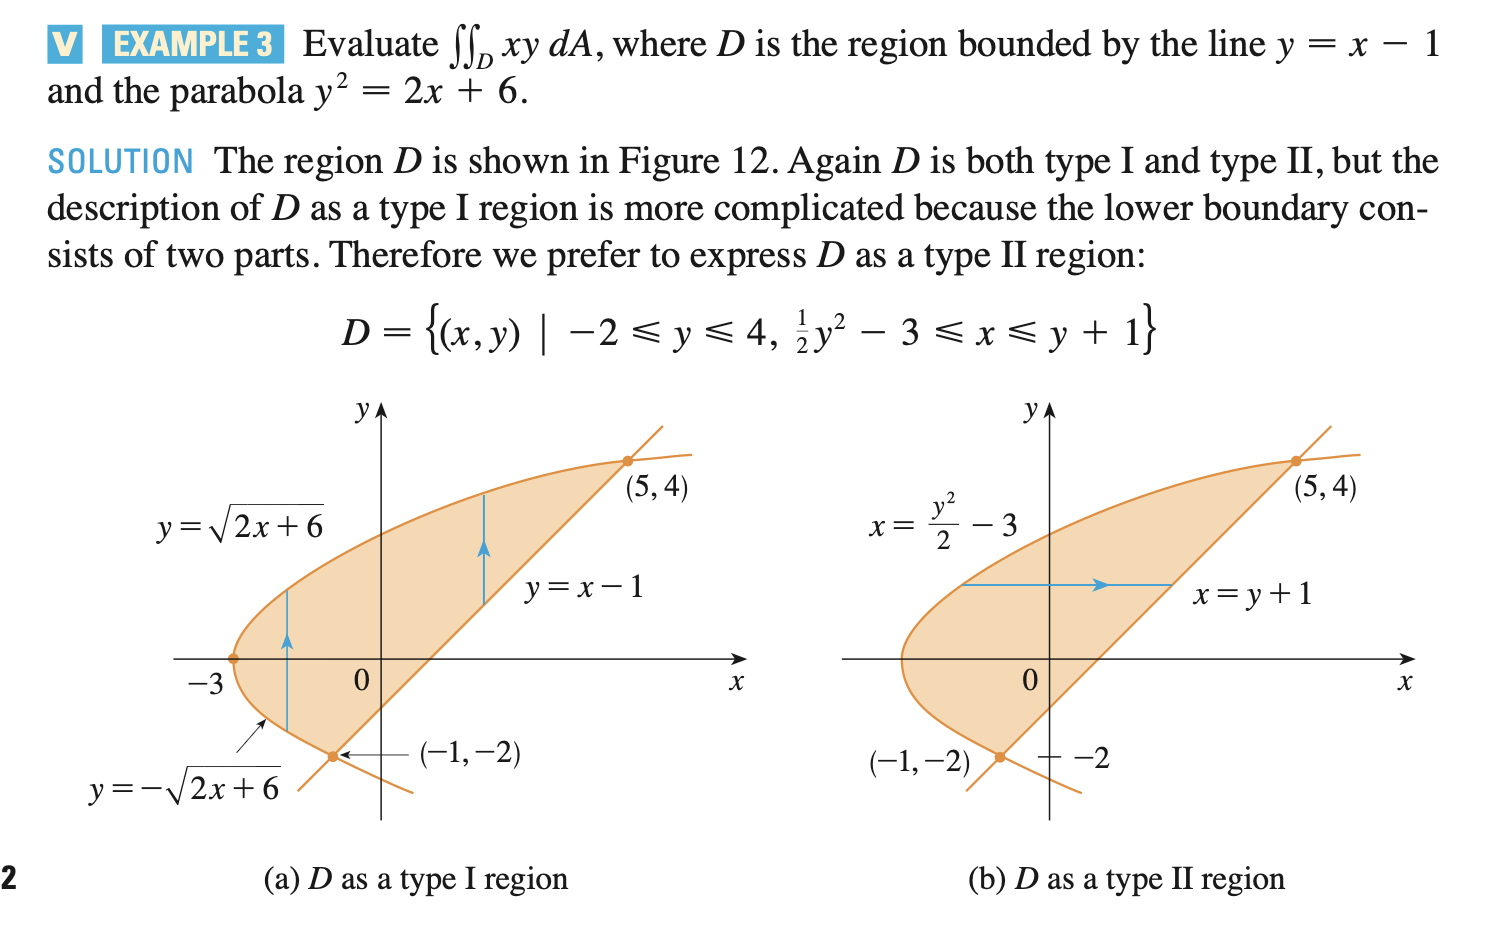
\includegraphics[width=0.5\linewidth]{TypeI&II_example.png}
            \label{fig:enter-label}
        \end{figure}
    \end{block}
\end{frame}

\begin{frame}{Polar Coordinates}
\frametitle{Polar Coordinates}

The polar coordinate system is a two-dimensional coordinate system in which each point on a plane is determined by a distance from a reference point and an angle from a reference direction.

\begin{columns}
    \begin{column}{0.5\textwidth}
        \textbf{Conversion Formulas}
        \vspace{1em}
        
        The relationships between Cartesian coordinates $(x, y)$ and polar coordinates $(r, \theta)$ are given by:
        
        \begin{align*}
            r^2 &= x^2 + y^2 \\
            x &= r \cos\theta \\
            y &= r \sin\theta
        \end{align*}
        
        Typically, we consider $r \ge 0$ and $0 \le \theta < 2\pi$.
        
    \end{column}
    \begin{column}{0.5\textwidth}
        \begin{tikzpicture}[scale=1.5]
            \draw[->] (-1.5,0) -- (1.5,0) node[right] {$x$};
            \draw[->] (0,-1.5) -- (0,1.5) node[above] {$y$};
            \draw[dashed] (0,0) -- (1,1);
            \node[above right] at (1,1) {$(x,y)=(r\cos\theta, r\sin\theta)$};
            \fill (1,1) circle (1pt);
            \draw (0,0) -- (1,1);
            \draw (0.3,0) arc (0:45:0.3);
            \node at (0.5,0.1) {$\theta$};
            \node[above, sloped] at (0.5,0.5) {$r$};
        \end{tikzpicture}
    \end{column}
\end{columns}

\end{frame}
\begin{frame}{Area Element: Cartesian vs. Polar}
\frametitle{Area Element: Cartesian vs. Polar}

The differential element of area $dA$ changes when we switch coordinate systems.

\begin{columns}
    \begin{column}{0.5\textwidth}
        \textbf{Cartesian Coordinates}
        \vspace{1em}
        The area element is a rectangle.
        
        \begin{center}
        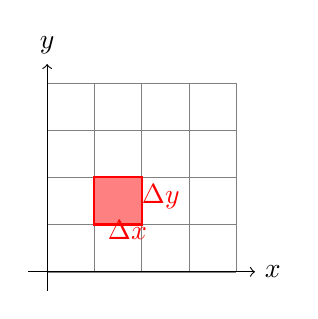
\begin{tikzpicture}[scale=1.2]
            \draw[step=0.5, gray, very thin] (0,0) grid (2,2);
            \draw[->] (-0.2,0) -- (2.2,0) node[right] {$x$};
            \draw[->] (0,-0.2) -- (0,2.2) node[above] {$y$};
            \fill[red!50!white, draw=red, thick] (0.5,0.5) rectangle (1,1);
            \node[right, red] at (0.9, 0.8) {$\Delta y$};
            \node[below, red] at (0.85, 0.65) {$\Delta x$};
        \end{tikzpicture}
        \end{center}
        
        As $\Delta x \to 0$ and $\Delta y \to 0$:
        $$ dA = dx \, dy $$
        
    \end{column}
    \begin{column}{0.5\textwidth}
        \textbf{Polar Coordinates}
        \vspace{1em}
        The area element is a "polar rectangle".
        
        \begin{center}
        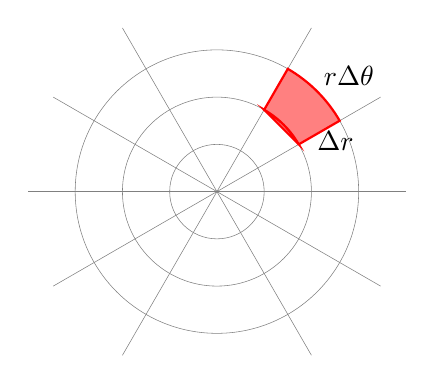
\begin{tikzpicture}[scale=1.2]
            \draw[gray, very thin] (0,0) circle (0.5);
            \draw[gray, very thin] (0,0) circle (1);
            \draw[gray, very thin] (0,0) circle (1.5);
            \draw[gray, very thin] (0:2) -- (180:2);
            \draw[gray, very thin] (30:2) -- (210:2);
            \draw[gray, very thin] (60:2) -- (240:2);
            \draw[gray, very thin] (120:2) -- (300:2);
            \draw[gray, very thin] (150:2) -- (330:2);
            \fill[red!50!white, draw=red, thick] (30:1) -- (60:1) arc (60:30:1) -- cycle;
            \fill[red!50!white, draw=red, thick] (30:1) -- (30:1.5) arc (30:60:1.5) -- (60:1) arc (60:30:1);
             %\draw[->, thick] (1.25,0.2) arc (20:40:1.25);
             \node[right] at (50:1.6) {$r\Delta\theta$};
             %\draw[->, thick] (45:1.05) -- (45:1.45);
             \node[above, sloped] at (15:1.3) {$\Delta r$};
        \end{tikzpicture}
        \end{center}
        
        The area is approximately $A \approx (r \, \Delta\theta) \Delta r$. As differentials:
        $ dA = r \, dr \, d\theta $
    \end{column}
\end{columns}

\end{frame}

\begin{frame}{Integration in Polar Coordinates}
\frametitle{Integration in Polar Coordinates}

A region $D$ defined in polar coordinates as:
$$ D = \{ (r, \theta) \mid r_1 \le r \le r_2, \, \theta_1 \le \theta \le \theta_2 \} $$
is called a \textbf{polar rectangle}.

\begin{center}
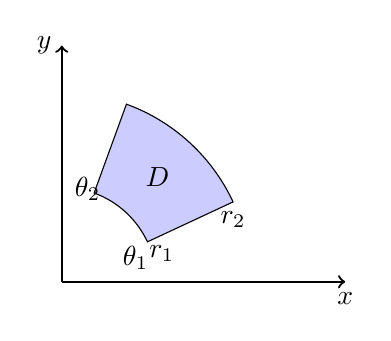
\begin{tikzpicture}[scale=1.2]
    % 坐标轴
    \draw[->, thick] (0,0) -- (3,0) node[below] {$x$};
    \draw[->, thick] (0,0) -- (0,2.5) node[left] {$y$};
    
    % 极坐标区域 D
    \fill[blue!20, draw=black] (25:1) arc (25:70:1) -- (70:2) arc (70:25:2) -- cycle;
    \node at (47.5:1.5) {$D$};
    
    % 角度标签
    %\draw (1.1,0) arc (25:70:1);
    \node[right] at (25:0.6) {$\theta_1$};
    %\draw (1.1,0) arc (0:70:0.8);
    \node[above] at (70:0.8) {$\theta_2$};
    
    % 半径标签
    \node[below] at (25:2) {$r_2$};
    \node[above left] at (5:1.3) {$r_1$};
\end{tikzpicture}
\end{center}

The integral over $D$ becomes:
$$ \iint_D f(x, y) \, dA = \int_{\theta_1}^{\theta_2} \int_{r_1}^{r_2} f(r\cos\theta, r\sin\theta) \, r \, dr \, d\theta $$
\end{frame}
% \begin{frame}{Change of Variables}
%     \begin{block}{Definition}
%         The \textbf{Jacobian} of the transformation $T$ given by $x=g(u,v)$ and $y=h(u,v)$ is 
%         \begin{equation*}
%             \dfrac{\partial(x,y)}{\partial(u,v)}=
%             \left|\begin{array}{cc}
%                 \frac{\partial x}{\partial u} & \frac{\partial x}{\partial v} \\
%                 \frac{\partial y}{\partial u} & \frac{\partial y}{\partial v}
%             \end{array}\right|
%             =\frac{\partial x}{\partial u}\frac{\partial y}{\partial v}-\frac{\partial x}{\partial v}\frac{\partial y}{\partial u}
%         \end{equation*}
%         Suppose that $T$ is a transformation whose \textbf{Jacobian} is \textbf{nonzero} and that maps a region $S$in the uv-plane onto a region $R$ in the xy-plane. $f$ is continuous on $R$ and that $R$ and $S$ are type I or type II plane regions. Suppose also that $T$ is one-to-one, except perhaps on the
% boundary of $S$. Then
%         \begin{equation*}
%             \iint_Rf(x,y)dA=\iint_Sf\big[x(u,v),y(u,v)\big]\Big| \dfrac{\partial(x,y)}{\partial(u,v)}\Big|dudv
%         \end{equation*}
%     \end{block}
% \end{frame}
\begin{frame}{Exercise}
    \textbf{Ex 6.1 }Evaluate$\iint_R(5-x)dA$, $R=\{(x,y)|0\leq x
    \leq 8,0\leq y\leq2\}$\\
    \par
    \textbf{Ex 6.2 }Evaluate $\iint_DxydA$, where $D$ is the region bounded by the line $y=x-1$ and the parabola $y^2=2x+6$.\\
    \textbf{Ex 6.3 }Express $D$ as a union of regions of type I or type II and evaluate the integral$\iint_D ydA$., where $D$ is the region bounded by the line $x=-1,y=-1,y=(x+1)^2,x=y-y^3$.\\
     \textbf{Ex 6.4} Use polar coordinates to combine the sum
     $\int_{1/\sqrt{2}}^1\int_{\sqrt{1-x^2}}^xxydydx+\int_1^{\sqrt{2}}\int_0^xxydydx+\int_{\sqrt{2}}^2\int_0^{\sqrt{4-x^2}}xydydx$ into one double integral. Then evaluate the double integral.\\
    \textbf{Ex 6.5} Evaluate $\iint_R(x+y)e^{x^2-y^2}dA$ by making an appropriate change of variables. $R$ is enclosed by the lines $x-y=0,x-y=2,x+y=0,x+y=3$.
\end{frame}
\begin{frame}{Answers}
    \textbf{6.1} 16\\
    \textbf{6.2} 36\\
    \textbf{6.3} $-\frac{2}{15}$\\
    \textbf{6.4} $\frac{15}{16}$\\
    \textbf{6.5} $\frac{1}{4}(e^6-7)$
\end{frame}


\section{Triple Integrals}
\begin{frame}[label=2]{Triple Integrals}
    \begin{enumerate}
  \item \textbf{Domain:}
  $$\mathcal{R} = [a, b] \times [c, d] \times [r,s].$$

  \item \textbf{Partial Integral:}
  $$\int_a^b f(x, y, z) \, dx$$

  \item \textbf{Iterated Integral:}
  $$\int_a^b \int_c^d \int_r^s f(x, y, z) \, dz \, dy \, dx = \int_a^b \left(\int_c^d \left(\int_r^s f(x, y, z) \, dz\right) \, dy\right) \, dx.$$

  \item \textbf{Theorem (Fubini’s Theorem):} The order of integration can be rearranged if $f$ is integrable over the region $\mathcal{R}$:
  $$\int \int \int_{\mathcal{R}} f \, dV = \int_a^b \int_c^d \int_r^s f(x, y, z) \, dz \, dy \, dx.$$

\end{enumerate}

\end{frame}

\begin{frame}
\frametitle{Problem: Find the Volume of a Solid}

% 使用 columns 环境来创建左右分栏
% [T] 选项使得两栏内容从顶部对齐
\begin{columns}[T]

    % --- 左侧栏:放置文本描述 ---
    \begin{column}{0.45\textwidth}
        \textbf{Problem}: Find the volume of the tetrahedron bounded by the planes:
        \vspace{1em}
        
        \begin{itemize}
            \item $x + 2y + z = 2$
            \item $x = 2y$
            \item $x = 0$
            \item $z = 0$
        \end{itemize}
        
        \vspace{1em}
        The volume $V$ is given by the integral:
        $$ V = \iiint_T dV $$
    \end{column}

    % --- 右侧栏:放置 TikZ 图片 ---
    \begin{column}{0.55\textwidth}
        \centering
        
        % 关键步骤 1: 在绘制前,先设置3D视角
        \tdplotsetmaincoords{70}{120}
        
        \resizebox{0.65\linewidth}{!}{%
            \begin{tikzpicture}
                % 关键步骤 2: 在一个 scope 环境中使用定义好的3D坐标系
                % 这样可以确保3D变换只作用于内部的图形
                \begin{scope}[tdplot_main_coords]
                    %--- 坐标轴 ---
                    \draw[->, thick] (0,0,0) -- (1.5,0,0) node[anchor=north east]{$x$};
                    \draw[->, thick] (0,0,0) -- (0,1.5,0) node[anchor=north west]{$y$};
                    \draw[->, thick] (0,0,0) -- (0,0,2.5) node[anchor=south]{$z$};
                
                    %--- 顶点 ---
                    \coordinate (V1) at (0,0,0);
                    \coordinate (V2) at (1,0.5,0);
                    \coordinate (V3) at (0,1,0);
                    \coordinate (V4) at (0,0,2);
                    
                    %--- 填充表面 ---
                    \fill[cyan!30, opacity=0.7] (V2) -- (V3) -- (V4) -- cycle;
                    \fill[cyan!15, opacity=0.5] (V1) -- (V2) -- (V3) -- cycle;
                    \fill[gray!20, opacity=0.5] (V1) -- (V4) -- (V3) -- cycle;
                
                    %--- 边 ---
                    \draw[thick, blue] (V2) -- (V3) -- (V4) -- cycle;
                    \draw[thick, blue] (V1) -- (V2);
                    \draw[thick, blue] (V1) -- (V3);
                    \draw[thick, blue] (V1) -- (V4);
                    
                    %--- 最终调整好的顶点标签 ---
                    \node[above right=3pt] at (V2) {\scriptsize(1, 1/2, 0)};
                    \node[below left=2pt] at (V3) {\scriptsize(0,1,0)};
                    \node[right=1pt] at (V4) {\scriptsize(0,0,2)};
                    \node[above left] at (V1) {\scriptsize O};
                \end{scope}
            \end{tikzpicture}%
        }
    \end{column}

\end{columns}
\end{frame}

\begin{frame}
\frametitle{Strategy: Project the Solid onto 2D Planes}
The key to setting up the integral is to understand the solid's "shadow" on the three coordinate planes. The complexity of these 2D regions often determines the difficulty of the integral.

\begin{columns}[T]

    % --- 第 1 栏:xy 平面投影 ---
    \begin{column}{0.33\textwidth}
        \textbf{On xy-plane ($R_{xy}$)}
        \centering
        \resizebox{\linewidth}{!}{%
            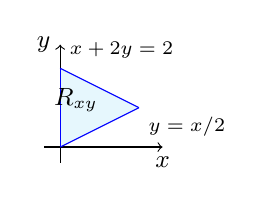
\begin{tikzpicture}[every node/.style={font=\small}]
                \fill[cyan!10] (0,0) -- (1,0.5) -- (0,1) -- cycle;
                \draw[->] (-0.2,0) -- (1.3,0) node[below]{$x$};
                \draw[->] (0,-0.2) -- (0,1.3) node[left]{$y$};
                \draw[blue] (0,0) -- (1,0.5) node[below right, black, font=\scriptsize]{$y=x/2$};
                \draw[blue] (1,0.5) -- (0,1) node[above right, black, font=\scriptsize]{$x+2y=2$};
                \draw[blue] (0,1) -- (0,0);
                \node at (0.2,0.6) {$R_{xy}$};
            \end{tikzpicture}%
        }
    \end{column}

    % --- 第 2 栏:xz 平面投影 ---
    \begin{column}{0.33\textwidth}
        \textbf{On xz-plane ($R_{xz}$)}
        \centering
        \resizebox{\linewidth}{!}{%
            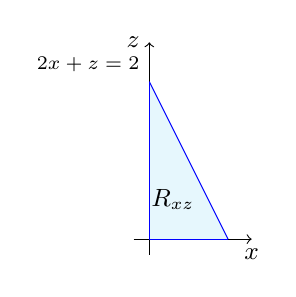
\begin{tikzpicture}[every node/.style={font=\small}]
                \fill[cyan!10] (1,0) -- (0,2) -- (0,0) -- cycle;
                \draw[->] (-0.2,0) -- (1.3,0) node[below]{$x$};
                \draw[->] (0,-0.2) -- (0,2.5) node[left]{$z$};
                \draw[blue] (1,0) -- (0,2) node[above left, black, font=\scriptsize]{$2x+z=2$};
                \draw[blue] (0,2) -- (0,0) -- (1,0);
                \node at (0.3,0.5) {$R_{xz}$};
            \end{tikzpicture}%
        }
    \end{column}

    % --- 第 3 栏:yz 平面投影 ---
    \begin{column}{0.33\textwidth}
        \textbf{On yz-plane ($R_{yz}$)}
        \centering
        \resizebox{\linewidth}{!}{%
            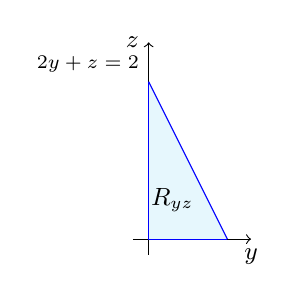
\begin{tikzpicture}[every node/.style={font=\small}]
                \fill[cyan!10] (1,0) -- (0,2) -- (0,0) -- cycle;
                \draw[->] (-0.2,0) -- (1.3,0) node[below]{$y$};
                \draw[->] (0,-0.2) -- (0,2.5) node[left]{$z$};
                \draw[blue] (1,0) -- (0,2) node[above left, black, font=\scriptsize]{$2y+z=2$};
                \draw[blue] (0,2) -- (0,0) -- (1,0);
                \node at (0.3,0.5) {$R_{yz}$};
            \end{tikzpicture}%
        }
    \end{column}

\end{columns}


\end{frame}

\begin{frame}
\frametitle{Orders based on $dz$ (Projection on $R_{xy}$)}
The inner integral is $\int_0^{2-x-2y} dz$. The outer double integral is over $R_{xy}$.

\begin{columns}[T]
    \begin{column}{0.5\textwidth}
        \alert<1>{Order $dz\,dy\,dx$ (No Split)}
        \begin{center}
        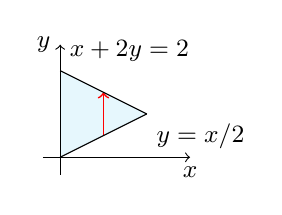
\begin{tikzpicture}[scale=1.1, every node/.style={font=\small}]
            \fill[cyan!10] (0,0) -- (1,0.5) -- (0,1) -- cycle;
            \draw[->, semithick, red] (0.5, 0.25) -- (0.5, 0.75); % Vertical strip
            \draw[->] (-0.2,0) -- (1.5,0) node[below]{$x$};
            \draw[->] (0,-0.2) -- (0,1.3) node[left]{$y$};
            \draw (0,0) -- (1,0.5) node[below right, black]{$y=x/2$};
            \draw (1,0.5) -- (0,1) node[above right, black]{$x+2y=2$};
        \end{tikzpicture}
        \end{center}
        $$ \int_0^1 \int_{x/2}^{(2-x)/2} \int_0^{2-x-2y} dz\,dy\,dx $$
    \end{column}
    \begin{column}{0.5\textwidth}
        \alert<1>{Order $dz\,dx\,dy$ (Requires Split)}
        \begin{center}
        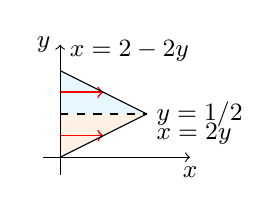
\begin{tikzpicture}[scale=1.1, every node/.style={font=\small}]
            \fill[orange!10] (0,0) -- (1,0.5) -- (0,0.5) -- cycle;
            \fill[cyan!10] (0,0.5) -- (1,0.5) -- (0,1) -- cycle;
            \draw[->, semithick, red] (0, 0.25) -- (0.5, 0.25);
            \draw[->, semithick, red] (0, 0.75) -- (0.5, 0.75);
            \draw[dashed] (0,0.5) -- (1,0.5) node[right, black]{$y=1/2$};
            \draw[->] (-0.2,0) -- (1.5,0) node[below]{$x$};
            \draw[->] (0,-0.2) -- (0,1.3) node[left]{$y$};
            \draw (0,0) -- (1,0.5) node[below right, black]{$x=2y$};
            \draw (1,0.5) -- (0,1) node[above right, black]{$x=2-2y$};
        \end{tikzpicture}
        \end{center}
        $$ \int_0^{1/2} \int_0^{2y}\int_0^{2-x-2y} dz\,dx\,dy $$ \\
        $$ + \int_{1/2}^1 \int_0^{2-2y} \int_0^{2-x-2y} dz\,dx\,dy $$
    \end{column}
\end{columns}
\end{frame}

\begin{frame}
\frametitle{Orders based on $dy$ (Projection on $R_{xz}$)}
The inner integral is $\int_{x/2}^{(2-x-z)/2} dy$. The outer double integral is over $R_{xz}$.

\begin{columns}[T]
    \begin{column}{0.5\textwidth}
        \alert<1>{Order $dy\,dz\,dx$ (No Split, Easiest)}
        \begin{center}
        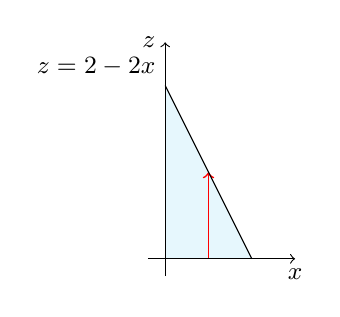
\begin{tikzpicture}[scale=1.1, every node/.style={font=\small}]
            \fill[cyan!10] (1,0) -- (0,2) -- (0,0) -- cycle;
            \draw[->, semithick, red] (0.5, 0) -- (0.5, 1);
            \draw[->] (-0.2,0) -- (1.5,0) node[below]{$x$};
            \draw[->] (0,-0.2) -- (0,2.5) node[left]{$z$};
            \draw (1,0) -- (0,2) node[above left, black]{$z=2-2x$};
        \end{tikzpicture}
        \end{center}
        $$ \int_0^1 \int_0^{2-2x} \int_{x/2}^{(2-x-z)/2} dy\,dz\,dx $$
    \end{column}
    \begin{column}{0.5\textwidth}
        \alert<1>{Order $dy\,dx\,dz$ (No Split)}
        \begin{center}
        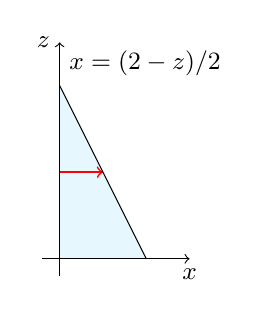
\begin{tikzpicture}[scale=1.1, every node/.style={font=\small}]
            \fill[cyan!10] (1,0) -- (0,2) -- (0,0) -- cycle;
            \draw[->, semithick, red] (0, 1) -- (0.5, 1);
            \draw[->] (-0.2,0) -- (1.5,0) node[below]{$x$};
            \draw[->] (0,-0.2) -- (0,2.5) node[left]{$z$};
            \draw (1,0) -- (0,2) node[above right, black]{$x=(2-z)/2$};
        \end{tikzpicture}
        \end{center}
        $$ \int_0^2 \int_0^{(2-z)/2} \int_{x/2}^{(2-x-z)/2} dy\,dx\,dz $$
    \end{column}
\end{columns}
\end{frame}

\begin{frame}
\frametitle{Complex Setup 1: Order $dx\,dy\,dz$}

\begin{columns}[T]
    % --- 左栏:图例和说明 ---
    \begin{column}{0.5\textwidth}
        Integrating with respect to $x$ first is complicated. Its upper bound is $\min(2y, 2-2y-z)$, forcing a split.
        \vspace{1em}
        
        The projection on the yz-plane, $R_{yz}$, is split by the line $\mathbf{4y+z=2}$.
        
        \begin{center}
        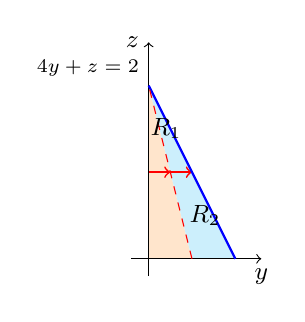
\begin{tikzpicture}[scale=1.1, every node/.style={font=\small}]
            \fill[orange!20] (0,0) -- (0.5,0) -- (0,2) -- (0,0);
            \fill[cyan!20] (0.5,0) -- (1,0) -- (0,2) -- (0.5,0);

            % Horizontal strips for dy-integration
            \draw[->, semithick, red] (0, 1) -- (0.25, 1);
            \draw[->, semithick, red] (0.25, 1) -- (0.5, 1);
            
            \draw[->] (-0.2,0) -- (1.3,0) node[below]{$y$};
            \draw[->] (0,-0.2) -- (0,2.5) node[left]{$z$};
            
            \draw[blue, thick] (1,0) -- (0,2);
            \draw[red, dashed] (0.5,0) -- (0,2) node[above left, black, font=\scriptsize]{$4y+z=2$};
            
            \node at (0.2,1.5) {$R_1$};
            \node at (0.65,0.5) {$R_2$};
        \end{tikzpicture}
        \end{center}
        
    \end{column}
    
    % --- 右栏:积分形式 ---
    \begin{column}{0.5\textwidth}
        \textbf{Setup for $dx\,dy\,dz$}
        \vspace{1em}
        
        This order splits the integral into two parts based on the horizontal integration strips.
        \vspace{1em}
        
        {\small
        $$ V = \underbrace{\int_0^2 \int_0^{(2-z)/4} \int_0^{2y} dx\,dy\,dz}_{\text{Volume over } R_1} $$
        $$ + \underbrace{\int_0^2 \int_{(2-z)/4}^{(2-z)/2} \int_0^{2-2y-z} dx\,dy\,dz}_{\text{Volume over } R_2} $$
        }
        
        
        
    \end{column}

\end{columns}

\end{frame}


\begin{frame}
\frametitle{Complex Setup 2: Order $dx\,dz\,dy$}

\begin{columns}[T]
    % --- 左栏:图例和说明 ---
    \begin{column}{0.5\textwidth}
        This order is even more complex, requiring the region to be broken into three separate triple integrals.
        \vspace{1em}
        
        The vertical integration strips for $dz$ cross over the splitting line $\mathbf{4y+z=2}$.
        
        \begin{center}
        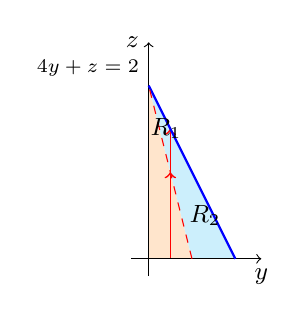
\begin{tikzpicture}[scale=1.1, every node/.style={font=\small}]
            \fill[orange!20] (0,0) -- (0.5,0) -- (0,2) -- cycle;
            \fill[cyan!20] (0.5,0) -- (1,0) -- (0,2) -- cycle;

            % Vertical strips for dz-integration
            \draw[->, semithick, red] (0.25, 0) -- (0.25, 1);
            \draw[->, semithick, red] (0.25, 1) -- (0.25, 2-2*0.25);
            
            \draw[->] (-0.2,0) -- (1.3,0) node[below]{$y$};
            \draw[->] (0,-0.2) -- (0,2.5) node[left]{$z$};
            
            \draw[blue, thick] (1,0) -- (0,2);
            \draw[red, dashed] (0.5,0) -- (0,2) node[above left, black, font=\scriptsize]{$4y+z=2$};
            
            \node at (0.2,1.5) {$R_1$};
            \node at (0.65,0.5) {$R_2$};
        \end{tikzpicture}
        \end{center}
        
    \end{column}
    
    % --- 右栏:积分形式 ---
    \begin{column}{0.5\textwidth}
        \textbf{Setup for $dx\,dz\,dy$}
        \vspace{1em}
        
        {\small
        $$ V = \underbrace{\int_0^{1/2} \int_0^{2-4y} \int_0^{2y} dx\,dz\,dy}_{\text{Bottom part of region}} $$
        $$ + \underbrace{\int_0^{1/2} \int_{2-4y}^{2-2y} \int_0^{2-2y-z} dx\,dz\,dy}_{\text{Middle part of region}} $$
        $$ + \underbrace{\int_{1/2}^1 \int_0^{2-2y} \int_0^{2-2y-z} dx\,dz\,dy}_{\text{Top part of region}} $$
        }
        
        
    \end{column}

\end{columns}
\end{frame}
\begin{frame}{Cylindrical Coordinates}
    \frametitle{Cylindrical Coordinates}
\begin{columns}
    % --- 左栏 ---
    \begin{column}{0.3\textwidth}
        \textbf{Cylindrical Coordinates} \\
        $\begin{cases}
            r &= \sqrt{x^2 + y^2} \\
            \theta &= \tan^{-1}\left(\frac{y}{x}\right) \\
            z &= z
        \end{cases}$
        \\
        $\begin{cases}
            x &= r\cos\theta \\
            y &= r\sin\theta \\
            z &= z
        \end{cases}$
    \end{column}
    
    % --- 右栏 ---
    \begin{column}{0.7\textwidth}
        \begin{figure}
            \centering
            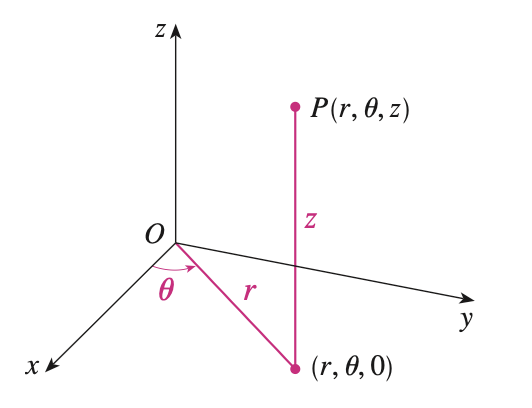
\includegraphics[width=0.45\linewidth]{cc_1.png}
        \end{figure}
        \begin{figure}
            \centering
            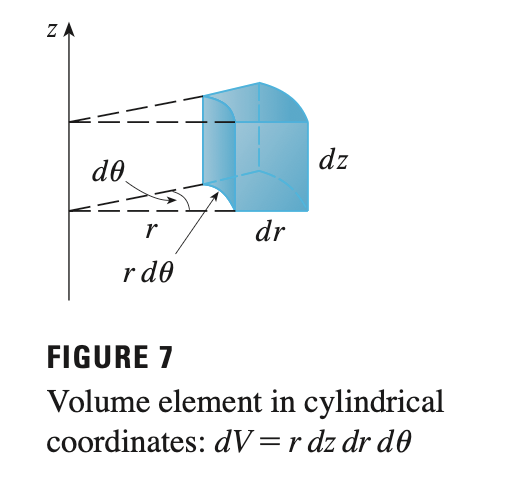
\includegraphics[width=0.45\linewidth]{cc_2.png}
        \end{figure}
    \end{column}
\end{columns}

\end{frame}

\begin{frame}
\frametitle{Example: Volume Using Cylindrical Coordinates}

\begin{block}{Problem}
    Calculate the volume of the solid enclosed by the paraboloid $z = x^2 + y^2$ and the plane $z = 4$.
\end{block}

\begin{columns}[T]
    % Left Column
    \begin{column}{0.5\textwidth}
        \begin{block}{1. Coordinate Transformation}
            This solid is rotationally symmetric, making it ideal for cylindrical coordinates.
            \begin{align*}
                x^2 + y^2 &= r^2 \\
                z &= z \\
                dV &= r \, dz \, dr \, d\theta
            \end{align*}
        \end{block}
    \end{column}
    
    % Right Column
    \begin{column}{0.5\textwidth}
        \begin{block}{2. Determine the Limits of Integration}
            \begin{itemize}
                \item \textbf{Range of $z$}: \\ $r^2 \le z \le 4$
                \item \textbf{Range of $r$}: \\ $0 \le r \le 2$
                \item \textbf{Range of $\theta$}: \\ $0 \le \theta \le 2\pi$
            \end{itemize}
        \end{block}
    \end{column}
\end{columns}

\begin{alertblock}{Next Step}
    With the coordinate system and limits defined, we can now set up the integral.
\end{alertblock}
\end{frame}


% --- Slide 2: Calculation ---
\begin{frame}
\frametitle{Example: Volume Using Cylindrical Coordinates (Cont.)}

\begin{block}{3. Set Up and Evaluate the Integral}
    The volume $V$ is given by the triple integral:
    \begin{align*}
        V &= \int_{0}^{2\pi} \int_{0}^{2} \int_{r^2}^{4} r \, dz \, dr \, d\theta \\
          &= \int_{0}^{2\pi} \int_{0}^{2} r [z]_{r^2}^{4} \, dr \, d\theta \\
          &= \int_{0}^{2\pi} \int_{0}^{2} r(4 - r^2) \, dr \, d\theta \\
          &= \int_{0}^{2\pi} \left[ 2r^2 - \frac{1}{4}r^4 \right]_{0}^{2} \, d\theta \\
          &= \int_{0}^{2\pi} 4 \, d\theta = 4[\theta]_{0}^{2\pi} = 8\pi
    \end{align*}
\end{block}

\end{frame}
\begin{frame}{Spherical Coordinates}
    \frametitle{Spherical Coordinates}
\begin{columns}
    % --- 左栏 ---
    \begin{column}{0.3\textwidth}
        \textbf{Spherical Coordinates} \\
$
\begin{cases}
    \rho &= \sqrt{x^2 + y^2 + z^2} \\
    \theta &= \tan^{-1}\left(\frac{y}{x}\right) \\
    \phi &= \cos^{-1}\left(\frac{z}{\rho}\right)
\end{cases}
$
\\
$
\begin{cases}
    x &= \rho\sin\phi\cos\theta \\
    y &= \rho\sin\phi\sin\theta \\
    z &= \rho\cos\phi
\end{cases}
$
    \end{column}
    
    % --- 右栏 ---
    \begin{column}{0.35\textwidth}
        \begin{figure}
            \centering
            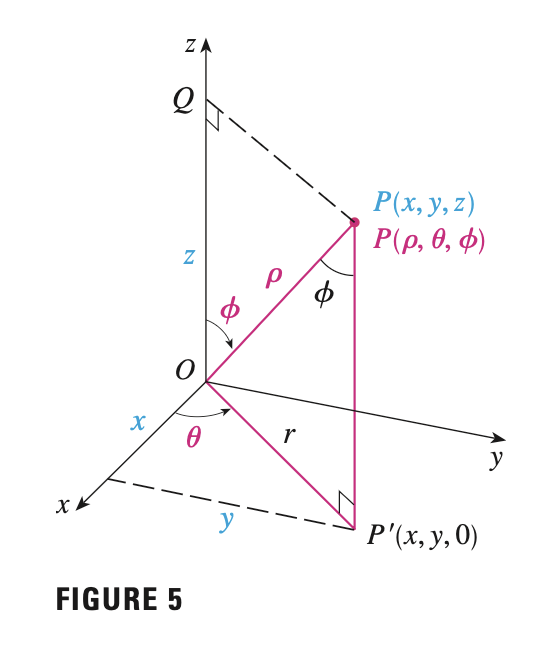
\includegraphics[width=0.8\linewidth]{sc_1.png}
        \end{figure}
    \end{column}
    \begin{column}{0.35\textwidth}
        \begin{figure}
            \centering
            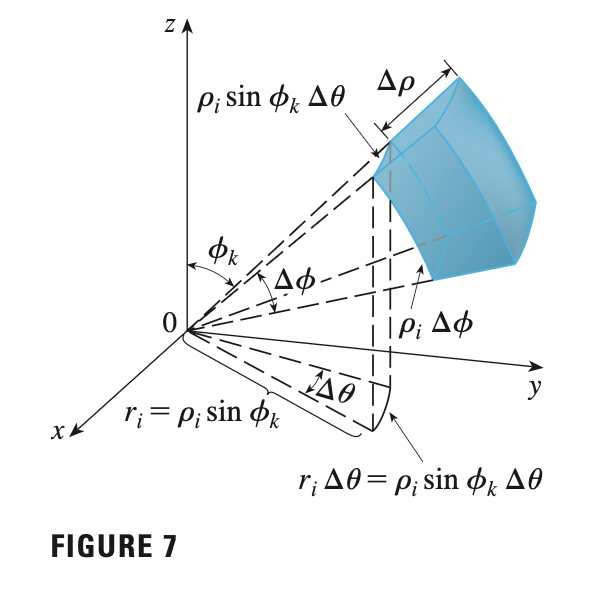
\includegraphics[width=0.8\linewidth]{sc_2.png}
        \end{figure}
    \end{column}
\end{columns}

\end{frame}
\begin{frame}
\frametitle{Example: Volume Using Spherical Coordinates}

\begin{block}{Problem}
    Calculate the volume of the part of the unit sphere $x^2+y^2+z^2 \le 1$ that lies in the first octant ($x\ge0, y\ge0, z\ge0$).
\end{block}

\begin{columns}[T]
    % Left Column
    \begin{column}{0.5\textwidth}
        \begin{block}{1. Coordinate Transformation}
            This problem involves a sphere, a perfect scenario for spherical coordinates.
            \begin{align*}
                 x^2+y^2+z^2 &= \rho^2 \\
                 dV &= \rho^2 \sin\phi \, d\rho \, d\phi \, d\theta
            \end{align*}
        \end{block}
    \end{column}
    
    % Right Column
    \begin{column}{0.5\textwidth}
        \begin{block}{2. Determine the Limits of Integration}
            \begin{itemize}
                \item \textbf{Range of $\rho$}: \\ $0 \le \rho \le 1$
                \item \textbf{Range of $\phi$}: \\ $0 \le \phi \le \pi/2$
                \item \textbf{Range of $\theta$}: \\ $0 \le \theta \le \pi/2$
            \end{itemize}
        \end{block}
    \end{column}
\end{columns}

\begin{alertblock}{Next Step}
    With the spherical limits defined, we can proceed to the integration.
\end{alertblock}

\end{frame}


% --- Slide 2: Calculation ---
\begin{frame}
\frametitle{Example: Volume Using Spherical Coordinates (Cont.)}

\begin{block}{3. Set Up and Evaluate the Integral}
    The volume $V$ is given by the triple integral:
    \begin{align*}
        V &= \int_{0}^{\pi/2} \int_{0}^{\pi/2} \int_{0}^{1} \rho^2 \sin\phi \, d\rho \, d\phi \, d\theta \\
          &= \int_{0}^{\pi/2} \int_{0}^{\pi/2} \sin\phi \left[ \frac{1}{3}\rho^3 \right]_{0}^{1} \, d\phi \, d\theta \\
          &= \frac{1}{3} \int_{0}^{\pi/2} \int_{0}^{\pi/2} \sin\phi \, d\phi \, d\theta \\
          &= \frac{1}{3} \int_{0}^{\pi/2} [-\cos\phi]_{0}^{\pi/2} \, d\theta \\
          &= \frac{1}{3} [\theta]_{0}^{\pi/2} = \frac{1}{3} \cdot \frac{\pi}{2} = \frac{\pi}{6}
    \end{align*}
\end{block}

\end{frame}

% \begin{frame}{Change of Variables}
%     \begin{block}{Theorem}
%         Let $\mathcal{R}$ and $\mathcal{S}$ be bounded regions in $\mathbb{R}^3$ that contain all of their boundary points. Let $T : \mathcal{D} \rightarrow \mathbb{R}^3$ where $\mathcal{D} \subset \mathbb{R}^3$ be an injective map that is onto and maps $\mathcal{S}$ in the $uvw$-plane to $\mathcal{R}$ in the $xyz$-plane. If $f(x, y, z)$ is continuous on $\mathcal{R}$, all of the components of $T$ have continuous partial derivatives and the Jacobian $JT(u, v, w)$ is never $0$ on $\mathcal{S}$, then
% \[
% \iiint_{\mathcal{R}} f(x, y, z) \, dx \, dy \, dz = \iiint_{\mathcal{S}} f(T(u, v, w)) \, \left| JT(u, v, w) \right| \, du \, dv \, dw.
% \]
%     \end{block}
% \end{frame}
% \begin{frame}{Frame Title}
%     The transformation \(T\) from cylindrical coordinates to rectangular coordinates is given by:
% \[ T(r, \theta,s) = \begin{bmatrix} r \cos \theta \\ r \sin \theta \\ s \end{bmatrix}^T. \]

% The transformation \(T\) from spherical coordinates to rectangular coordinates is given by:
% \[ T(\rho, \theta, \phi) = \begin{bmatrix} \rho \sin \phi \cos \theta \\ \rho \sin \phi \sin \theta \\ \rho \cos \phi \end{bmatrix}^T. \]
% \end{frame}

% \begin{frame}{Remark}
%     The Jacobian \( J \) of the transformation from cylindrical to rectangular coordinates is:
% \[ J(r, \theta, s) = r. \]

% The Jacobian \( J \) of the transformation from spherical to rectangular coordinates is:
% \[ J(\rho, \theta, \phi) = -\rho^2 \sin \phi. \]
% \end{frame}
\begin{frame}{Exercise}
    \textbf{Exercise 6.6} Find the mass of the pyramid with base in the plane $z = -6$ and sides
formed by the three planes $y = 0$, $y - x = 4$ and $2x + y + z = 4$
if the density of the solid is given by $\delta(x, y, z) = y$. \\
    \textbf{Exercise 6.7} Find the volume of the region bounded by $z = x + y$, $x + y = 5$,
where $(x, y) \in [0, 5] \times [0, 5]$, and the planes $x = 0$, $y = 0$, and $z = 0$. \\

    \textbf{Exercise 6.8} Evaluate the integral
\[
\int_{-\sqrt{3}}^{\sqrt{3}} \int_{-\sqrt{3-x^2}}^{\sqrt{3-x^2}} \int_{1}^{4-x^2-y^2} \frac{1}{z^2} \, dz \, dy \, dx.
\] 
\end{frame}
\begin{frame}{Answers - 6.6}
    We calculate the triple integral by
\[
\int_{0}^{6} \int_{y-4}^{5-\frac{y}{2}} \int_{-6}^{4-2x-y} y \, dz \, dx \, dy = 243.
\]
\end{frame}
\begin{frame}{Answers - 6.7}
    Here we calculate the volume $V$ of the region $E$ using a triple integral:
\[
V = \iiint_E \, dV = \int_0^5 \int_0^{5-x} \int_0^{x+y} \, dz \, dy \, dx = \frac{125}{3}.
\]

\end{frame}
\begin{frame}{Answers - 6.8}
    Use cylindrical coordinates. The transformation is given by:
\begin{align*}
\begin{cases}
x = r \cos \theta \\
y = r \sin \theta \\
z = z
\end{cases}
\Rightarrow
\begin{cases}
0 \leq r \leq \sqrt{3} \\
0 \leq \theta \leq 2\pi \\
1 \leq z \leq 4 - r^2
\end{cases}
\end{align*}
and $|J(r, \theta, z)| = r$.

Therefore, the integral
\[
\int_{-\sqrt{3}}^{\sqrt{3}} \int_{-\sqrt{3-x^2}}^{\sqrt{3-x^2}} \int_{1}^{4-x^2-y^2} \frac{1}{z^2} \, dz \, dy \, dx
\]
becomes
\[
\int_{0}^{2\pi} \int_{0}^{\sqrt{3}} \int_{1}^{4-r^2} \frac{1}{z^2} r \, dz \, dr \, d\theta 
\]
\[ 
= 2\pi \int_{0}^{\sqrt{3}} \left( r - \frac{r}{4 - r^2} \right) dr =(3-ln 4) \pi.
\]
\end{frame}
% \section{Vector Field}
    
% \begin{frame}[label=3]{Vector Field}
%     \begin{block}{Definition}
%         A vector field on two (or three) dimensional space is a function $\boldsymbol{F}$ that assigns to each point $(x, y)$ (or $(x, y, z)$) a two (or three) dimensional vector given by $\boldsymbol{F}(x, y)$ (or $\boldsymbol{F}(x, y, z)$).
%     \end{block}
%     The standard notation for the function $\boldsymbol{F}$ is,
% \[
% \boldsymbol{F}(x, y) = P(x, y) \boldsymbol{i} + Q(x, y) \boldsymbol{j}
% \]
% \[
% \boldsymbol{F}(x, y, z) = P(x, y, z) \boldsymbol{i} + Q(x, y, z) \boldsymbol{j} + R(x, y, z) \boldsymbol{k}
% \]
% \end{frame}
% \begin{frame}{Gradient Fields}
% \begin{block}{Definition}
%     If $f$ is a scalar function of two variables, then its gradient $\nabla f$(or grad $f$) is defined by
%     \begin{equation*}
%         \nabla f(x,y)=f_x(x,y)\boldsymbol{i}+f_y(x,y)\boldsymbol{j}
%     \end{equation*}
% \end{block}
    
% \end{frame}

% \begin{frame}{Exercise}
%     \textbf{Ex 6.9} Find the gradient vector field of following functions.
%     \begin{enumerate}
%         \item $f(x,y,z)=\sqrt{x^2+y^2+z^2}$
%         \item $f(x,y)=ln(1+x^2+y^2)$
%     \end{enumerate}
% \end{frame}

\begin{frame}{\textcolor{green!30!black}{end}}
    \begin{center}
        \LARGE Thank you!
    \end{center}
\end{frame}



\end{document}

\begin{frame}{Integral Domain}
    \begin{block}{Definition}
         Let $\mathcal{R} = [a, b] \times [c, d]$ and $u_1 : \mathcal{R} \rightarrow \mathbb{R}$, $u_2 : \mathcal{R} \rightarrow \mathbb{R}$ be continuous functions. Let $D$ be a region in $\mathbb{R}^2$ that is contained in $\mathcal{R}$ ($D \subset \mathcal{R}$). Let $\mathcal{R}$ be the solid region whose projection onto the $xy$-plane is $D$ and that is bounded on the $z$-axis by functions $u_1(x, y)$ and $u_2(x, y)$, i.e., 
\[
\mathcal{R} = \{(x, y, z) \in \mathbb{R}^3 \mid (x, y) \in D \text{ and } u_1(x, y) \leq z \leq u_2(x, y)\}.
\]
A region of this form is said to be a \emph{Type I solid region}.
    \end{block}
    Let $\mathcal{R} = [a, b] \times [c, d]$ and $u_1 : \mathcal{R} \rightarrow \mathbb{R}$, $u_2 : \mathcal{R} \rightarrow \mathbb{R}$ be continuous functions. Let $D$ be a region in $\mathbb{R}^2$ that is contained in $\mathcal{R}$ ($D \subset \mathcal{R}$). Let $\mathcal{R}$ be the solid region whose projection onto the $xy$-plane is $D$ and that is bounded on the $z$-axis by functions $u_1(x, y)$ and $u_2(x, y)$, i.e., 
\[
\mathcal{R} = \{(x, y, z) \in \mathbb{R}^3 \mid (x, y) \in D \text{ and } u_1(x, y) \leq z \leq u_2(x, y)\}.
\]
A region of this form is said to be a \emph{Type I solid region}.
\end{frame}
